
\documentclass[pdf]{beamer}

\mode<presentation>{}

\usetheme{CambridgeUS}

\usepackage[utf8]{inputenc}
\usepackage{tikz}
\usetikzlibrary{positioning}
\usetikzlibrary{calc}

\usepackage{listings}
\lstset{emph={new, val, trait}, emphstyle=\color{red} }
\title{Tower Defense}
\author{Alexis Laouar, R\'emi Oudin, K\'evin Le Run}

\begin{document}

\begin{frame}
  \titlepage
\end{frame}

\section{Fonctionnalit\'es}

\subsection{Réseau TCP}
\begin{frame}
    \frametitle{\subsecname}
    \begin{itemize}
        \item Mise en place d'un réseau Serveur-Clients
        \item Multi-threading
        \item Sérialisation des instances
    \end{itemize}
\end{frame}

\subsection{Gestion des différents rôles}
\begin{frame}
    \frametitle{\subsecname}
    \begin{itemize}
        \item Mise en place de \emph{Strategy}
        \item Le même code, sauf à quelques endroits
        \item Permet une réduction des communications
    \end{itemize}
\end{frame}

\subsection{Règles du jeu}
\begin{frame}
    \frametitle{\subsecname}
    \begin{itemize}
        \item Chaque joueur attaque et défend.
        \item On attaque avec des spawners.
        \item On défend avec des tours.
    \end{itemize}
\end{frame}

\section{Architecture}

\subsection{MVC}

\begin{frame}
  \frametitle{Serveur-Clients}
  \begin{figure}[h]
    \centering
    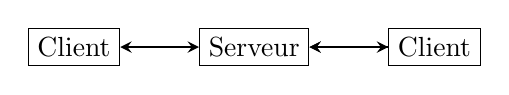
\begin{tikzpicture}[
      elementblock/.style={draw,rectangle},
      node distance=1cm]
      % Blocks
      \node[elementblock]                                     (server)      {Serveur};
      \node[elementblock,right=of server]                       (client1){Client};
      \node[elementblock,left=of server](client2)     {Client};

      % Arrows
      \draw[         -{stealth},thick] (client1) edge (server);
      \draw[{stealth}-{stealth},thick] (client1) edge (server) (server) edge (client2);

    \end{tikzpicture}
  \end{figure}
\end{frame}

\section{Une State Machine pour les menus}

\begin{frame}
  \frametitle{Les menus}
    \begin{itemize}
        \item Pour gérer les connexions
        \item Pour gérer les options
        \item Pour savoir qui on est
    \end{itemize}
\end{frame}

\begin{frame}
    \frametitle{La state machine}
    \begin{itemize}
        \item Chaque menu est un état du jeu
        \item Le jeu est un état.
        \item État différent si serveur ou client.
    \end{itemize}
\end{frame}

\section{La GUI}
\begin{frame}
    \frametitle{Des arbres pour l'affichage}
    \begin{itemize}
        \item La fenêtre est est la racine
        \item Chaque élément est un fils.
        \item C'est récursif
    \end{itemize}
\end{frame}

\begin{frame}[fragile]
    \frametitle{Un exemple}
    \lstinputlisting{tdcomponent.scala}
\end{frame}
\section{Conclusion}

\end{document}
